%\documentclass{article}
\documentclass[preview=true]{standalone}
% !TeX spellcheck = en-GB
\usepackage{graphicx,fullpage,tikz}
\newcommand{\dir}{Figures}
\graphicspath{{\dir/}}
\pagestyle{empty}
\begin{document}
\centering
before \texttt{checkAndDuplicatePeriodicParticles}

%\setlength{\unitlength}{1cm}
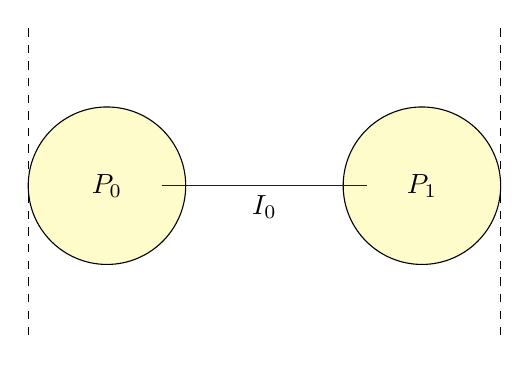
\begin{tikzpicture}[scale=2,
 interaction/.style ={-,draw=blue,shorten >=.8cm,shorten <=.8cm},
 wall/.style ={-,dashed,draw=black},
 particle/.style ={fill=yellow!20!white, draw=black}
 ]
%draw particle 0
\draw[particle] (0.5,1) circle (.5) node  {$P_0$};
%draw particle 1
\draw[particle] (2.5,1) circle (.5) node  {$P_1$};
%draw periodic walls
\draw[wall] (0,2) -- (0,0);
\draw[wall] (3,2) -- (3,0);
%draw interaction 0
\draw[interaction] (0.45,1) -- (2.55,1)  node [midway, below] {$I_0$};
\end{tikzpicture}

during \texttt{computeForces}

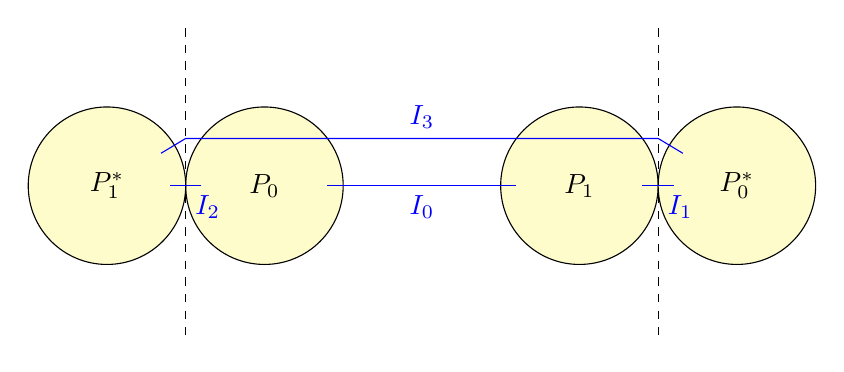
\begin{tikzpicture}[scale=2,
 interaction/.style ={-,draw=blue,shorten >=.8cm,shorten <=.8cm},
 wall/.style ={-,dashed,draw=black},
 particle/.style ={fill=yellow!20!white, draw=black}
 ]
%draw particle 0
\draw[particle] (0.5,1) circle (.5) node  {$P_0$};
%draw particle 1
\draw[particle] (2.5,1) circle (.5) node  {$P_1$};
%draw particle 2
\draw[particle] (3.5,1) circle (.5) node  {$P_0^*$};
%draw particle 3
\draw[particle] (-0.5,1) circle (.5) node  {$P_1^*$};
%draw periodic walls
\draw[wall] (0,2) -- (0,0);
\draw[wall] (3,2) -- (3,0);
%draw interaction 0
\draw[interaction] (0.5,1) -- (2.5,1)  node [blue,midway, below] {$I_0$};
%draw interaction 1
\draw[interaction] (3.5,1) -- (2.5,1)  node [blue,midway, below right] {$I_1$};
%draw interaction 2
\draw[interaction] (0.5,1) -- (-.5,1)  node [blue,midway, below right] {$I_2$};
%draw interaction 3
\draw[interaction] (3.5,1) -- (3,1.3) -- (0,1.3)-- (-0.5,1)  node [blue,above] at (1.5,1.3) {$I_3$};
\end{tikzpicture}

after \texttt{removeDuplicatePeriodicParticles} \\
(the interaction with between the real particle with the lower index \\
and the ghost particle of the higher index gets preserved)

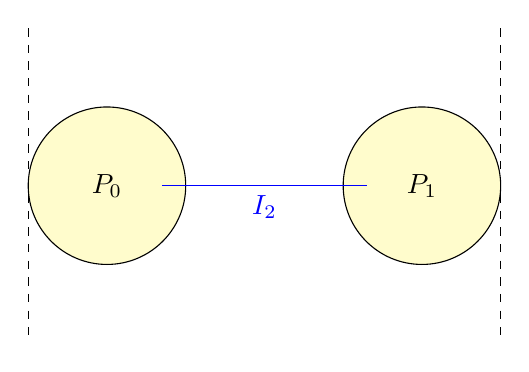
\begin{tikzpicture}[scale=2,
 interaction/.style ={-,draw=blue,shorten >=.8cm,shorten <=.8cm},
 wall/.style ={-,dashed,draw=black},
 particle/.style ={fill=yellow!20!white, draw=black}
 ]
%draw particle 0
\draw[particle] (0.5,1) circle (.5) node  {$P_0$};
%draw particle 1
\draw[particle] (2.5,1) circle (.5) node  {$P_1$};
%draw periodic walls
\draw[wall] (0,2) -- (0,0);
\draw[wall] (3,2) -- (3,0);
%draw interaction 0
\draw[interaction] (0.45,1) -- (2.55,1)  node [midway, below,blue] {$I_2$};
\end{tikzpicture}

\end{document}